\section{Introduction}

Power/performance trade offs are well established compromises in the design of all embedded systems \cite{das2016reliability}. In both hardware and software domains, there is a great deal of formal and empirical knowledge which guides system architects towards optimal design time decisions, and myriad runtime operation modes (i.e., power saving modes) controlled locally or remotely \cite{senni2016non}. Approximate computing promises unprecedented power savings by introducing a trade off between power and another dimension: accuracy \cite{mittal2016survey}. For applications resiliant to innacurate computations \cite{xu2016approximate}, or where there isn't a single golden result \cite{venkataramani2016approximate}, approximate computing methods can improve traditional design strategies for power reduction: essential in the dark silicon era \cite{mitra2017power}.
\par Despite its promise, approximate computing is still an immature technology: a formal model of the impact of approximations on other design metrics does not yet exist \cite{venkataramani2015approximate}. Hence, most approximate computing applications require two premises to be implemented successfully: (a) adequate test data are available, to correctly model the accuracy impact of approximations \cite{yazdanbakhsh2017axbench}; and, (b) approximations are performed iteratively at design time, in order to meet the required power/accuracy goals, and remain static throughoput deployment \cite{nepal2016automated}.
\par This is a stark contrast to performance/power trade offs, where well established benchmark suites offer near total coverage of application scenarios \cite{henning2000spec}: in approximate computing, test data that allows adequate modeling of accuracy is often unavailable. In performance/power trade offs, systems can self-tune their operation based on load and run time parameters to dynamically adjust metrics \cite{isci2003runtime}. In approximate computing, approximations are static: mainly because there is no trusted method to determine if accuracy suffices, without access to ground truth \cite{chippa2013analysis}. In this paper, we tackle this problem:  adjusting the level of approximations at run time, for signal processing applications. Our hypothesis states that prior knowledge about processed data can guide built-in approximation engines, dynamically modifying the level of approximations whilst ensuring that accuracy suffices for the required task.
\par Specifically, this paper offers the following contributions:

\begin{itemize}
\item	We introduce the concept of prior knowledge-guided approximations. This represents a statistical measure of approximation impact, unlike test data-based empirical measures prevalent in the state of the art \cite{zhang2014approxit}.
\item	We introduce a model of run time approximations, which use prior knowledge to ensure that accuracy suffices, without access to ground truth, unlike iterative comparisons to ground truth prevalent in the state of the art \cite{han2013approximate}.
\item 	We describe and evaluate a proof of concept of our approach, using an Extended Kalman Filter for motion tracking \cite{kulikov2016accurate}, where we have prior knowledge about the target's motion. 
\end{itemize}

\par The remainder of this paper is organized as follows: Section \ref{learning} describes a top level view of our methodology, explaining how prior knowledge can guide approximations dynamically. Section \ref{} describes a case study of our proposed method, where prior knowledge is used to dynamically adjust the approximations applied to an Extended Kalman Filter for tracking. Section \ref{} describes our experimental setup and the obtained results. Finally, Section \ref{} presents our conclusions and future work. 


\begin{figure}[tb]
  \centering
  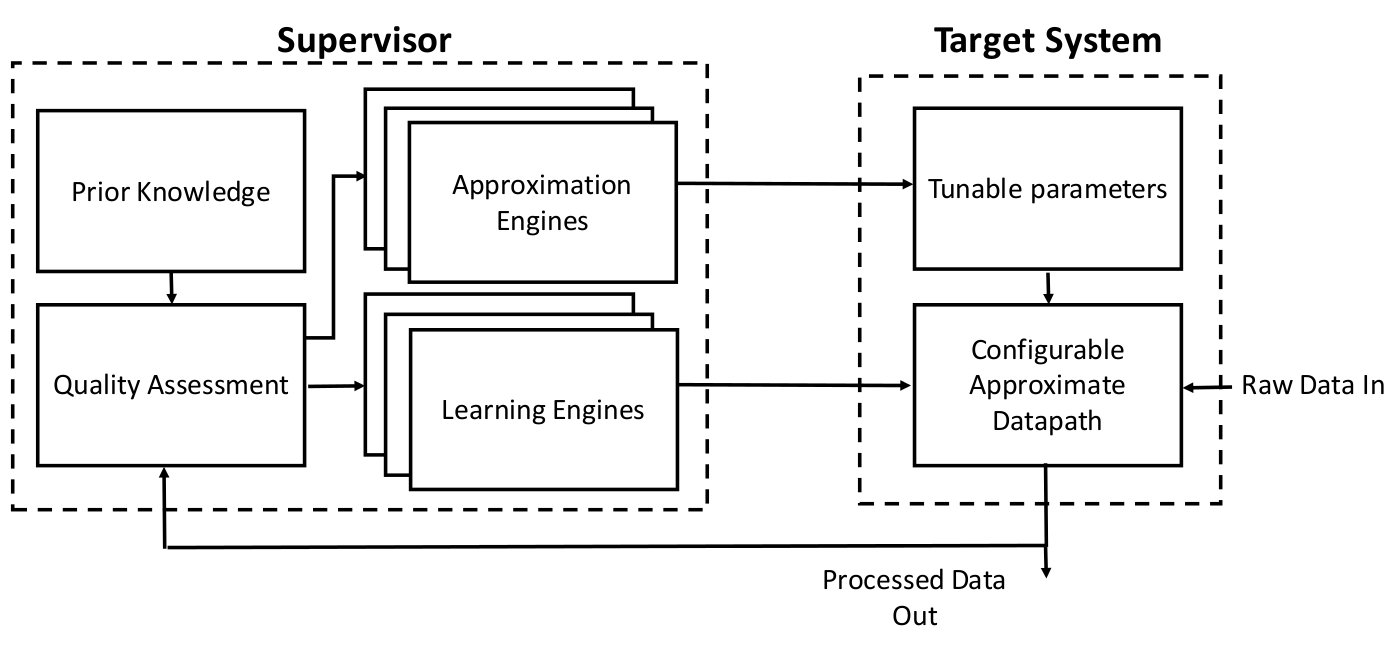
\includegraphics[width=\columnwidth]{img/block_diagram.png}
  \caption{Block diagram}
  \label{fig:block_diagram}
\end{figure}
